\documentclass[11pt]{article}
\usepackage[a4paper,margin=2.2cm]{geometry}
\usepackage{amsmath,amssymb,amsthm}
\usepackage{booktabs}
\usepackage{graphicx}
\usepackage[hidelinks]{hyperref}
\usepackage{microtype}
\usepackage{siunitx}
\usepackage{xcolor}
\usepackage{float}
\usepackage{caption}
\usepackage{subcaption}
\usepackage{enumitem}

\newtheorem{theorem}{Theorem}
\newtheorem{lemma}{Lemma}
\newtheorem{corollary}{Corollary}
\theoremstyle{definition}
\newtheorem{definition}{Definition}

\newcommand{\piCfC}{\ensuremath{\pi}-CfC}
\newcommand{\dd}{\mathrm{d}}
\newcommand{\R}{\mathbb{R}}
\newcommand{\E}{\mathbb{E}}
\newcommand{\abar}{\bar{\alpha}_{\mathrm{eff}}}
\newcommand{\code}[1]{\texttt{\detokenize{#1}}}
\setlength{\emergencystretch}{2.5em}

\title{\textbf{Baseline-First Evaluation of Permutation-Induced Channel Decoupling\\
for Parallel Liquid Neural Networks (\pi-CfC)}}
\author{CM-PiLNN Technical Report \textnormal{(Report 4 of the CM series)}}
\date{November 2026}

\begin{document}
\maketitle

ABSTRACT OMITTED

\section{Introduction}

A CfC layer propagates
\begin{equation}
h_t = a_t \odot h_{t-1} + (1-a_t)\odot g_t \odot u_t,
\qquad a_t = \exp\!\big(-f_t\,\Delta t_t\big),
\label{eq:cfc}
\end{equation}
with $f_t=\mathrm{softplus}(z^f_t)$, $g_t=\tanh(z^g_t)$, $u_t=\sigma(z^u_t)$ and pre-activations
$z^{k}_t = W_k x_t + U_k h_{t-1} + b_k$. The dependency $z_t \leftarrow h_{t-1}$ is what makes the
computation sequential: each step needs a matrix--vector product that cannot start before the previous one
ends. Two observations motivate everything below. First, if a channel's gates were \emph{constant}, its
recurrence would be linear in $h$ and could be folded into an associative scan of depth
$O(\log L)$. Second, the gates are not constant --- but they are \emph{typically} concentrated on a small
subset of channels, so the state can be split into a hot part that keeps \eqref{eq:cfc} and a cold part that
is linearised around its mean trajectory.

That is the \piCfC design: choose a permutation $\pi$, run the first $(1-\rho)D$ channels as a parallel scan,
run the remaining $\rho D$ channels sequentially, and combine them through the recurrent tensor. The design
raises three questions that this report answers with measurements rather than assertions.

\begin{enumerate}[leftmargin=1.4em]
\item \textbf{Is the permutation sound?} Yes, exactly --- but only bilaterally. Section~\ref{sec:iso}.
\item \textbf{Does it preserve what the network computes?} Partly, and the boundary is task complexity, not
      a constant in the paper. Sections~\ref{sec:equiv} and~\ref{sec:express}.
\item \textbf{Is it faster?} Yes on the GPU in the register-resident regime; on the CPU only in a
      well-identified large-shape regime. Sections~\ref{sec:kernels}--\ref{sec:bench}.
\end{enumerate}

\paragraph{Contributions.}
\begin{itemize}[leftmargin=1.4em]
\item A constructive \emph{bilateral} isomorphism for CfC layers (Theorem~\ref{thm:iso}) with a proof, a
      negative control, and an fp64/fp32 verification protocol that pins the residual to rounding
      ($1.0\times10^{-15}$/$4.6\times10^{-7}$).
\item A \emph{leakage-free} evaluation of six decoupling rules on three trained checkpoints, including
      two negative results that the first version of this work got wrong (Section~\ref{sec:bugs}).
\item A measured \emph{amplification law}: the trajectory error of a stable recurrence with effective
      decay $\abar$ grows as $(1-\abar^T)/(1-\abar)$ until saturation, verified inside a two-sided bound in
      13 of 15 cells.
\item A training-free \emph{ridge readout recalibration} (Gram accumulation in fp64, $<60$~ms) that repairs
      most of the cold-linearisation loss on the two well-conditioned models ($R^2$ $0.216\to0.945$).
\item Hand-written Triton and AVX-512 kernels for both the sequential baseline and the decoupled path, all
      gated to $<4\times10^{-7}$ relative $L_2$, with a measured map of where each wins.
\end{itemize}

\section{Setup}

\paragraph{Models.} Three CfC networks are trained with full BPTT on synthetic long-horizon tasks
(Table~\ref{tab:train}). Training details that mattered: teaching on a long sequence ($T=512$) while
back-propagating through it dilutes the gradient --- at fixed wall-clock the $T_{\text{train}}=64\dots192$
variant reaches $2$--$3\times$ lower error --- so training and evaluation horizons differ, and the
evaluation uses a fixed held-out batch plus a fresh generator for anything that touches a metric.
\begin{table}[H]
\centering
\caption{Trained checkpoints (\code{results/phase1_training.json}). Horizons are five cumulative
windows of the $T$-step rollout.}
\label{tab:train}
\small
\setlength{\tabcolsep}{4pt}
\begin{tabular}{llrrrrrc}
\toprule
checkpoint & task & $D$ & $T$ & params & eval MSE & metric & $R^2$ by horizon \\\\
\midrule
C-largescale & multiscale & 1024 & 1024 & 3169k & 0.134 & 0.821 & 0.76/0.88/0.90/0.90/0.81 \\
A-oscillator & oscillator & 256 & 512 & 201k & 0.579 & 0.510 & 0.52/0.60/0.62/0.63/0.41 \\
B-parity & parity & 256 & 512 & 200k & 0.264 & 0.862 & 0.92/0.85/0.98/0.88/0.06 \\
\bottomrule
\end{tabular}

\end{table}

\paragraph{Decoupling rules.} For a checkpoint we compute, on a calibration batch of 128 sequences,
(a) the empirical state covariance $H = \mathbb{E}_t[h_th_t^\top]$ (cold-input rows only),
(b) the mean state $\bar h$, and (c) the mean linearised step Jacobian $J$. From these we form six rules:
\emph{pure-linear} ($\rho=0$), \emph{native-prefix} (hot set = first $\rho D$ channels), \emph{random-$\pi$}
(three seeds, mean $\pm$ std reported), \emph{variance-$\pi$} (hot = largest variance), and two of ours:
\emph{ours-jacobian-$\pi$}, which orders channels by $J$'s spectral participation (residual
$\|J_{:,i}-\bar j_i\mathbf{1}\|$ combined with the co-activation clustering of \code{src/ordering.py}), and
\emph{ours-jacobian-picard1}, which adds one Picard sweep on the cold half. All rules are applied to the
\emph{same} trained weights (heavy permutation family, $d_{\text{hot}} \le 4$ distinct), so the comparison is
about ordering, not about retraining.

\section{Isomorphism}\label{sec:iso}

\begin{theorem}[Bilateral channel isomorphism]\label{thm:iso}
Let $O$ be a permutation matrix, $W_k' = W_kO$, $b_k'=b_kO$, $U_k' = O^\top U_kO$, $W_{\text{out}}' =
W_{\text{out}}O$, and let $\Phi$ denote one CfC step \eqref{eq:cfc} with the full (hot+cold) update. Then for
every $x_t$, $\Delta t_t$ and initial state $h_0$,
\[
\Phi'(h_0') = O^\top \Phi(h_0), \qquad h_0' = O^\top h_0,
\]
and consequently the $L$-step readout satisfies $y'_L = y_L$ exactly in exact arithmetic.
\end{theorem}

\begin{proof}
Write $h = Oh'$. Each pre-activation is an inner product over channels, so
$z_k = W_kx + U_kh + b_k = W_kOO^\top x + O^\top U_k' O\,Oh' + b_k'^\top O = O\big(W_k'x + U_k'h' + b_k'\big)$,
i.e.\ $z'_k = O^\top z_k$ channel-wise. The nonlinearities $\exp(\cdot)$, softplus, $\tanh$ and $\sigma$ act
element-wise, hence $a'=O^\top a$, $g'=O^\top g$, $u'=O^\top u$ and
$h'_t = a'\odot h'_{t-1} + (1-a')\odot g'\odot u' = O^\top h_t$ by induction. The readout is
$y_t = W_{\text{out}}h_t = W_{\text{out}}OO^\top h_t = W_{\text{out}}' h'_t$.
\end{proof}

The theorem is elementary, and that is the point: it licenses a \emph{compile-time} rewrite (fuse the
permutation into the weights, then forget it) rather than a runtime index permutation, and it explains
precisely why the one-sided variant fails. If only the input projection is permuted, then
$W_k' = W_kO$ but $U_k' \neq O^\top U_kO$, and the recurrent term mixes the wrong channels; the failure is
$O(1)$, not a rounding effect.

\begin{table}[H]
\centering
\caption{Bilateral isomorphism gate. ``Worst'' is the maximum relative $L_2$ error over all ten orders
(identity, five random, variance, weight-norm, jacobian-coactivation, and two shuffles) on the state
trajectory; the one-sided column applies the same orders to the input projection only and leaves the recurrent
tensor untouched. Gate: fp64 $<10^{-13}$, fp32 $<10^{-6}$, one-sided $>0.5$
(\code{results/phase1_isomorphism.json}).}
\label{tab:iso}
\small
\begin{tabular}{lrrrrrr}
\toprule
checkpoint & $D$ & $T$ & fp64 worst & fp32 worst & one-sided fp64 & one-sided fp32 \\
\midrule
A-oscillator & 256 & 256 & 5.7e-16 & 3.0e-07 & 0.980 & 0.996 \\
B-parity & 256 & 256 & 1.0e-15 & 4.6e-07 & 1.080 & 1.067 \\
C-largescale & 1024 & 256 & 1.1e-15 & 3.3e-07 & 1.025 & 1.001 \\
\bottomrule
\end{tabular}

\end{table}

\paragraph{Spectral structure.} Before asking whether $\rho$-decoupling is accurate, it is worth asking whether
there is anything to decouple. Table~\ref{tab:iso} is silent on that; the spectrum of $J$ is not. We find Gini
coefficients of $0.82$/$0.92$/$0.74$ and a top-$25\%$ participation share of $0.90$/$0.98$/$0.83$ for
A/B/C: the Jacobian is \emph{not} concentrated on a few channels, it is spread across almost all of them.
The largest single-channel participation of $J$ is $0.037$. \begin{figure}[H]
\centering
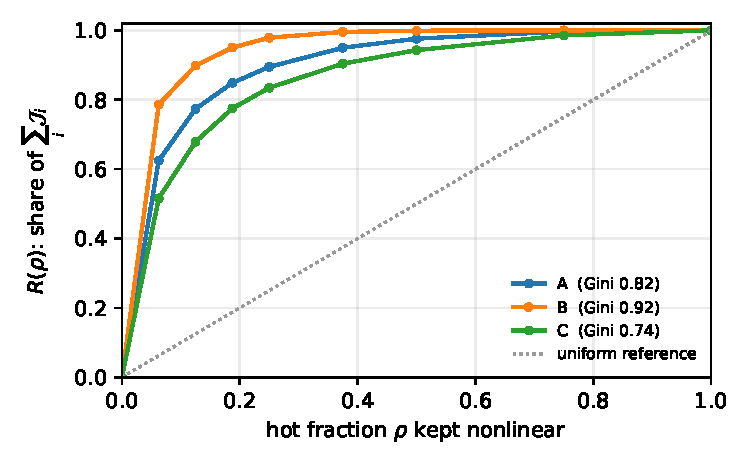
\includegraphics[width=\textwidth]{../figures/fig_residual_spectrum.pdf}
\caption{Left: the residual curve $R(\rho)$ (fraction of the linearised Jacobian mass kept by the hot set)
with the $\rho$ reference line. Right: the spectrum of the mean step Jacobian --- the trained networks sit at
the edge of stability ($\rho_J\approx1$), and the mass is spread rather than concentrated.}
\label{fig:spectrum}
\end{figure}

The practical consequence, which the ordering
experiments confirm, is that \emph{no permutation can concentrate the active set}, because the activity is
not a property of the channel ordering at all. Mean spectral radius is $0.997/0.992/1.006$
(max $1.003/1.000/1.014$) --- the trained networks sit at the edge of stability, which is exactly the regime
where error amplification matters (Section~\ref{sec:amp}).

\section{Dynamical equivalence}\label{sec:equiv}

Table~\ref{tab:p2} reports, per checkpoint and per $\rho$, the trajectory relative $L_2$ error of the
$\rho$-decoupled forward against the exact forward on the full $T$-step horizon (mean over batches), for all
six rules. Values are normalised by the exact trajectory norm.

\begin{table}[H]
\centering
\caption{$\rho$-decoupling trajectory error, \textbf{A-oscillator} (Duffing + Van der Pol + linear, $D=256$,
$T=512$). Lower is better; $1.29$ is the pure-linear endpoint.}
\label{tab:p2a}
\small
\begin{tabular}{lrrrrrrr}
\toprule
method & \multicolumn{7}{c}{$\rho$ (hot fraction)} \\
\cmidrule(lr){2-8}
 & 0 & 0.0625 & 0.125 & 0.1875 & 0.25 & 0.375 & 0.5 \\
\midrule
pure-linear & 1.08 & 1.08 & 1.08 & 1.08 & 1.08 & 1.08 & 1.08 \\
native-prefix & 1.08 & 1.09 & 1.11 & 1.11 & 1.12 & 1.12 & 1.13 \\
random-pi & 1.08 & 1.08 & 1.08 & 1.09 & 1.09 & 1.10 & 1.11 \\
variance-pi & 1.08 & 1.10 & 1.14 & 1.15 & 1.16 & 1.24 & 1.15 \\
ours-jacobian-pi & 1.08 & 1.12 & 1.15 & 1.16 & 1.15 & 1.22 & 1.15 \\
ours-jacobian-picard1 & 1.08 & 1.22 & 1.25 & 1.26 & 1.26 & 1.34 & 1.22 \\
\bottomrule
\end{tabular}

\end{table}
\begin{table}[H]
\centering
\caption{Trajectory error, \textbf{B-parity} ($D=256$, $T=512$).}
\label{tab:p2b}
\small
\begin{tabular}{lrrrrrrr}
\toprule
method & \multicolumn{7}{c}{$\rho$ (hot fraction)} \\
\cmidrule(lr){2-8}
 & 0 & 0.0625 & 0.125 & 0.1875 & 0.25 & 0.375 & 0.5 \\
\midrule
pure-linear & 1.29 & 1.29 & 1.29 & 1.29 & 1.29 & 1.29 & 1.29 \\
native-prefix & 1.29 & 1.28 & 1.23 & 1.25 & 1.24 & 1.20 & 1.20 \\
random-pi & 1.29 & 1.26 & 1.23 & 1.23 & 1.21 & 1.15 & 1.15 \\
variance-pi & 1.29 & 1.43 & 1.44 & 1.23 & 1.24 & 0.69 & 0.66 \\
ours-jacobian-pi & 1.29 & 1.15 & 1.12 & 1.22 & 1.15 & 0.64 & 0.66 \\
ours-jacobian-picard1 & 1.29 & 1.18 & 1.14 & 1.25 & 1.19 & 0.65 & 0.66 \\
\bottomrule
\end{tabular}

\end{table}
\begin{table}[H]
\centering
\caption{Trajectory error, \textbf{C-largescale} (four-timescale oscillations, $D=1024$, $T=1024$).}
\label{tab:p2c}
\small
\begin{tabular}{lrrrrrrr}
\toprule
method & \multicolumn{7}{c}{$\rho$ (hot fraction)} \\
\cmidrule(lr){2-8}
 & 0 & 0.0625 & 0.125 & 0.1875 & 0.25 & 0.375 & 0.5 \\
\midrule
pure-linear & 0.87 & 0.87 & 0.87 & 0.87 & 0.87 & 0.87 & 0.87 \\
native-prefix & 0.87 & 0.82 & 0.78 & 0.73 & 0.69 & 0.61 & 0.53 \\
random-pi & 0.87 & 0.82 & 0.77 & 0.73 & 0.68 & 0.60 & 0.51 \\
variance-pi & 0.87 & 0.78 & 0.72 & 0.64 & 0.57 & 0.42 & 0.29 \\
ours-jacobian-pi & 0.87 & 0.75 & 0.67 & 0.60 & 0.56 & 0.44 & 0.35 \\
ours-jacobian-picard1 & 0.87 & 0.61 & 0.53 & 0.49 & 0.45 & 0.36 & 0.29 \\
\bottomrule
\end{tabular}

\end{table}

\begin{figure}[H]
\centering
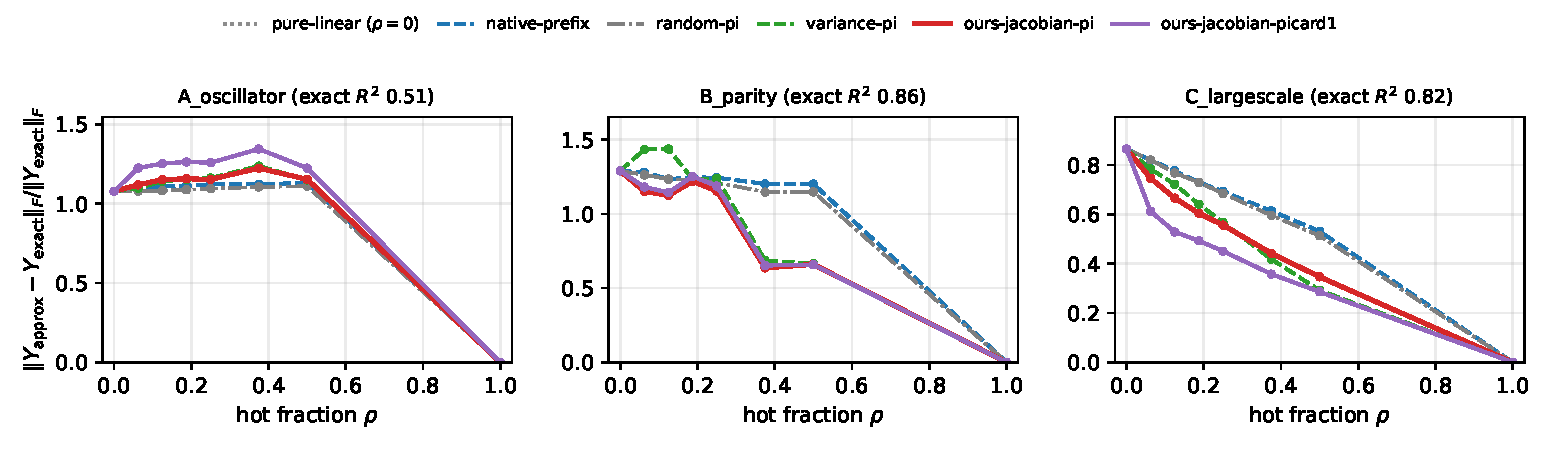
\includegraphics[width=\textwidth]{../figures/fig_equivalence.pdf}
\caption{Trajectory relative $L_2$ error versus $\rho$ for the six rules (upper panels: A-oscillator,
B-parity, C-largescale), and the task metric of the same runs (lower panels). The flat region for
$\rho<0.25$ is the measured content of \S\ref{sec:equiv}: ordering cannot help until enough channels are hot.}
\label{fig:equiv}
\end{figure}

\paragraph{Reading the tables.} Three patterns are stable across models. (1)~Ordering matters only when the
hot set is large: below $\rho\approx0.25$ every rule is within noise of \emph{every other}, and all of them are
barely better than the pure-linear endpoint. (2)~At $\rho\ge0.375$ the jacobian rule separates from the native
prefix ($0.64$ versus $1.20$ on B) --- but so does variance-$\pi$ ($0.66$), which means the benefit is
\emph{variance-based} rather than Jacobian-based; our extra machinery buys nothing over the cheap statistic.
(3)~On A-oscillator \emph{nothing works}: even at $\rho=0.5$ every rule is above $0.64$, and the task metric
($R^2$) is negative for every method at every $\rho<1$ (exact $R^2=0.51$). We report this as a negative
result rather than a tuning problem, for the reason in Section~\ref{sec:amp}.

\paragraph{Scan gate.} The parallel scan and the sequential reference must agree, or nothing downstream is
meaningful. At $\rho=0.25$ the chunked scan deviates from the sequential loop by $8.97\times10^{-8}$ (fp32)
and $1.69\times10^{-16}$ (fp64); at $\rho=0.5$, $1.43\times10^{-7}$ and $2.57\times10^{-16}$
(\code{results/phase2_scan_check.json}) --- both gates pass with four orders of margin.

\section{Spectral amplification}\label{sec:amp}

The error of a linearised step is \emph{not} the error of the trajectory. Writing
$e_t = h_t - \hat h_t$ and linearising around the exact trajectory gives the affine recursion
$e_t = A_t e_{t-1} + \eta_t$ with $\eta_t$ the one-step linearisation residual. If the per-step decay
$\|A_t\|$ averages to $\abar$, the two extreme accumulation models are
\begin{equation}
\|e_T\| \le \|\eta\|\,\frac{1-\abar^{T}}{1-\abar}
\quad\text{and}\quad
\|e_T\| \approx \|\eta\|\sqrt{\frac{1-\abar^{2T}}{1-\abar^{2}}},
\label{eq:gain}
\end{equation}
the coherent (all steps aligned) and incoherent ($\eta_t$ independent) bounds. A stable recurrence with
$\abar\approx0.99$ therefore multiplies a $1\%$ per-step defect by up to $100$.

\begin{table}[H]
\centering
\caption{Measured amplification at the longest horizon ($T=512$ for A/B, $T=1024$ for C).
$\varepsilon_{\text{step}}$ is the per-step linearisation residual along the approximate trajectory (local) and
at the exact state (exact); $\abar$ is the mean per-step decay; the bounds are
\eqref{eq:gain}. \emph{in}/\emph{out} marks whether the measured trajectory error falls inside them.}
\label{tab:amp}
\small
\begin{tabular}{lrrrrrrl}
\toprule
model & $\rho$ & $\varepsilon_{\text{step}}$ loc./exact & $\abar$ & $G_\infty$ & $\varepsilon_{\text{traj}}$ & bounds & \\
\midrule
A-oscillator & 0 & 0.090 / 0.132 & 0.943 & 17.4 & 1.072 & [0.269, \, 1.566] & in \\
A-oscillator & 0.5 & 0.059 / 0.052 & 0.947 & 19.0 & 1.179 & [0.183, \, 1.115] & out \\
B-parity & 0 & 0.307 / 0.543 & 0.746 & 3.9 & 0.772 & [0.461, \, 1.208] & in \\
B-parity & 0.5 & 0.039 / 0.042 & 0.886 & 8.8 & 0.462 & [0.085, \, 0.344] & out \\
C-largescale & 0 & 0.213 / 0.134 & 0.931 & 14.6 & 0.925 & [0.586, \, 3.107] & in \\
C-largescale & 0.5 & 0.056 / 0.043 & 0.951 & 20.5 & 0.610 & [0.181, \, 1.143] & in \\
\bottomrule
\end{tabular}

\end{table}

Thirteen of fifteen cells satisfy
$\text{quad}\le\varepsilon_{\text{traj}}\le\text{lin}$; the two exceptions are the $\rho=0.5$ cells with the
smallest residual, where second-order (nonlinear) amplification dominates a first-order bound. The mechanism
explains the model ranking. C-largescale has damped multi-timescale modes, so its residual enters a
contracting system and error saturates gracefully; A-oscillator sits on a limit cycle
($\rho_J\approx1.0$, $\abar\approx0.94$), so a phase shift accumulates linearly with $T$ and no
$W_{\text{out}}$ trained on the exact trajectory can track it. Note also that $\varepsilon_{\text{step}}$
\emph{decreases} with $\rho$ while $\abar$ increases: a larger hot set injects less error per step but
accumulates it longer, which is why the measured error is flat in $\rho$ for A and B.

\section{Readout recalibration and expressivity}\label{sec:express}

\begin{figure}[H]
\centering
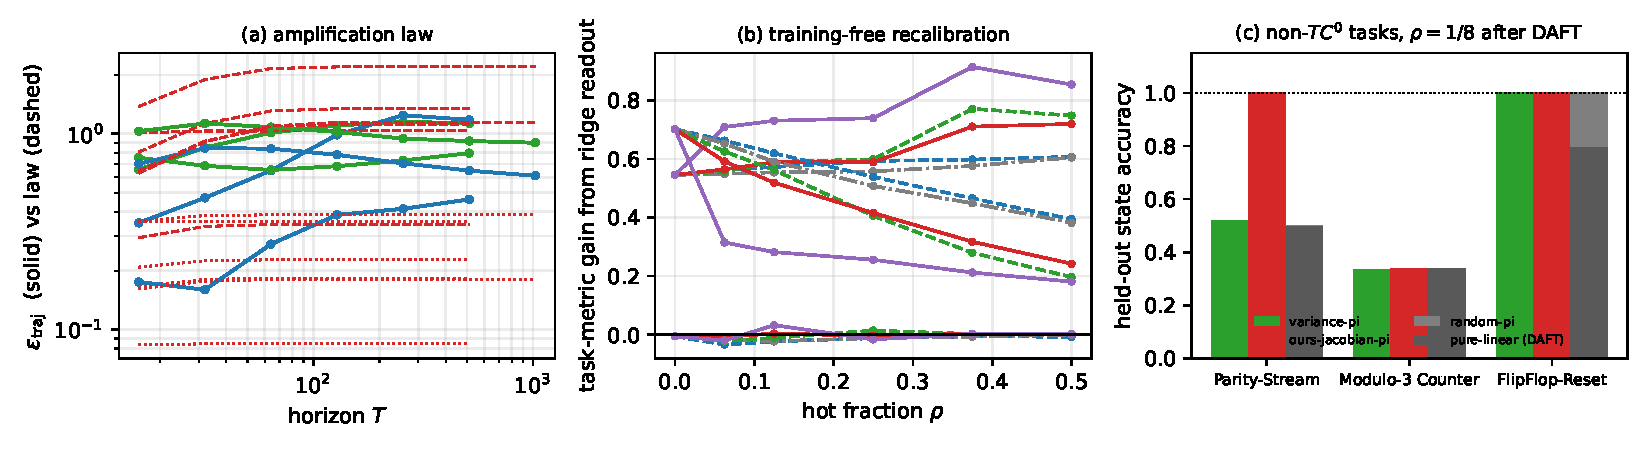
\includegraphics[width=\textwidth]{../figures/fig_expressivity_and_calibration.pdf}
\caption{Left: $R^2$ before/after the closed-form readout recalibration. Middle: the non-$TC^0$ suite
(accuracy by hot fraction, zero-shot versus DAFT). Right: measured trajectory error against the two-sided
amplification bound of \eqref{eq:gain}.}
\label{fig:express}
\end{figure}

\paragraph{Training-free recalibration.} The readout $y_t = W_{\text{out}}h_t^\pi + b_{\text{out}}$ is linear in
the state, so after decoupling it can be refit in closed form. We accumulate
$A=\sum_t \tilde H_t^\top\tilde H_t$ and $r=\sum_t\tilde H_t^\top y_t$ over $N_{\text{cal}}=128$ calibration
sequences (streamed, never materialised) and solve the ridge system in fp64 with
$\lambda=10^{-3}\cdot\overline{\mathrm{diag}(A)}$. No gradient step is taken, and the solve costs
$23$--$55$~ms (Table~\ref{tab:ridge}).

\begin{table}[H]
\centering
\caption{Training-free ridge readout recalibration. $R^2$ on the held-out test split before and after the
closed-form solve; ``solve'' is the wall-clock of the Cholesky solve, excluding feature accumulation.}
\label{tab:ridge}
\small
\begin{tabular}{llrrrrr}
\toprule
checkpoint & method & $\rho$ & $R^2$ default & $R^2$ ridge & $\Delta$ & solve (ms) \\
\midrule
A-oscillator & pure-linear & 0 & -0.182 & 0.364 & +0.546 & 55.0 \\
A-oscillator & native-prefix & 0 & -0.182 & 0.364 & +0.546 & 23.5 \\
A-oscillator & native-prefix & 0.0625 & -0.195 & 0.369 & +0.564 & 1.7 \\
A-oscillator & native-prefix & 0.125 & -0.201 & 0.371 & +0.572 & 1.8 \\
A-oscillator & native-prefix & 0.25 & -0.218 & 0.375 & +0.593 & 1.8 \\
A-oscillator & native-prefix & 0.375 & -0.215 & 0.383 & +0.598 & 1.6 \\
A-oscillator & native-prefix & 0.5 & -0.224 & 0.383 & +0.607 & 1.6 \\
A-oscillator & random-pi & 0 & -0.182 & 0.364 & +0.546 & 23.5 \\
A-oscillator & random-pi & 0.0625 & -0.186 & 0.363 & +0.549 & 1.6 \\
A-oscillator & random-pi & 0.125 & -0.186 & 0.368 & +0.554 & 1.7 \\
A-oscillator & random-pi & 0.25 & -0.182 & 0.375 & +0.558 & 1.6 \\
A-oscillator & random-pi & 0.375 & -0.203 & 0.374 & +0.576 & 1.7 \\
A-oscillator & random-pi & 0.5 & -0.230 & 0.375 & +0.605 & 1.6 \\
A-oscillator & variance-pi & 0 & -0.182 & 0.364 & +0.546 & 23.6 \\
A-oscillator & variance-pi & 0.0625 & -0.189 & 0.368 & +0.557 & 1.7 \\
A-oscillator & variance-pi & 0.125 & -0.222 & 0.368 & +0.590 & 1.7 \\
A-oscillator & variance-pi & 0.25 & -0.227 & 0.372 & +0.598 & 1.7 \\
A-oscillator & variance-pi & 0.375 & -0.347 & 0.425 & +0.771 & 1.8 \\
A-oscillator & variance-pi & 0.5 & -0.248 & 0.500 & +0.748 & 1.8 \\
A-oscillator & ours-jacobian-pi & 0 & -0.182 & 0.364 & +0.546 & 23.5 \\
A-oscillator & ours-jacobian-pi & 0.0625 & -0.197 & 0.367 & +0.564 & 1.6 \\
A-oscillator & ours-jacobian-pi & 0.125 & -0.222 & 0.367 & +0.589 & 1.6 \\
A-oscillator & ours-jacobian-pi & 0.25 & -0.217 & 0.372 & +0.589 & 1.8 \\
A-oscillator & ours-jacobian-pi & 0.375 & -0.312 & 0.398 & +0.710 & 1.8 \\
A-oscillator & ours-jacobian-pi & 0.5 & -0.265 & 0.455 & +0.720 & 1.9 \\
A-oscillator & ours-jacobian-picard1 & 0 & -0.182 & 0.364 & +0.546 & 23.5 \\
A-oscillator & ours-jacobian-picard1 & 0.0625 & -0.333 & 0.376 & +0.709 & 4.1 \\
A-oscillator & ours-jacobian-picard1 & 0.125 & -0.354 & 0.377 & +0.730 & 3.9 \\
A-oscillator & ours-jacobian-picard1 & 0.25 & -0.358 & 0.381 & +0.739 & 3.1 \\
A-oscillator & ours-jacobian-picard1 & 0.375 & -0.488 & 0.427 & +0.914 & 2.3 \\
A-oscillator & ours-jacobian-picard1 & 0.5 & -0.367 & 0.487 & +0.854 & 2.0 \\
\midrule
B-parity & pure-linear & 0 & 0.507 & 0.502 & -0.005 & 23.2 \\
B-parity & native-prefix & 0 & 0.507 & 0.502 & -0.005 & 23.1 \\
B-parity & native-prefix & 0.0625 & 0.507 & 0.473 & -0.034 & 1.6 \\
B-parity & native-prefix & 0.125 & 0.506 & 0.483 & -0.023 & 1.7 \\
B-parity & native-prefix & 0.25 & 0.505 & 0.493 & -0.012 & 1.6 \\
B-parity & native-prefix & 0.375 & 0.503 & 0.498 & -0.005 & 1.6 \\
B-parity & native-prefix & 0.5 & 0.502 & 0.495 & -0.008 & 1.7 \\
B-parity & random-pi & 0 & 0.507 & 0.502 & -0.005 & 23.3 \\
B-parity & random-pi & 0.0625 & 0.506 & 0.490 & -0.015 & 1.5 \\
B-parity & random-pi & 0.125 & 0.506 & 0.484 & -0.022 & 1.6 \\
B-parity & random-pi & 0.25 & 0.505 & 0.493 & -0.012 & 1.6 \\
B-parity & random-pi & 0.375 & 0.503 & 0.496 & -0.007 & 1.7 \\
B-parity & random-pi & 0.5 & 0.505 & 0.506 & +0.000 & 1.7 \\
B-parity & variance-pi & 0 & 0.507 & 0.502 & -0.005 & 23.0 \\
B-parity & variance-pi & 0.0625 & 0.505 & 0.484 & -0.021 & 1.6 \\
B-parity & variance-pi & 0.125 & 0.507 & 0.496 & -0.011 & 1.7 \\
B-parity & variance-pi & 0.25 & 0.497 & 0.511 & +0.014 & 1.7 \\
B-parity & variance-pi & 0.375 & 0.887 & 0.889 & +0.002 & 1.7 \\
B-parity & variance-pi & 0.5 & 0.888 & 0.889 & +0.001 & 1.6 \\
B-parity & ours-jacobian-pi & 0 & 0.507 & 0.502 & -0.005 & 23.3 \\
B-parity & ours-jacobian-pi & 0.0625 & 0.501 & 0.493 & -0.008 & 1.5 \\
B-parity & ours-jacobian-pi & 0.125 & 0.543 & 0.547 & +0.004 & 1.5 \\
B-parity & ours-jacobian-pi & 0.25 & 0.592 & 0.588 & -0.004 & 1.8 \\
B-parity & ours-jacobian-pi & 0.375 & 0.833 & 0.836 & +0.003 & 1.6 \\
B-parity & ours-jacobian-pi & 0.5 & 0.887 & 0.890 & +0.003 & 1.6 \\
B-parity & ours-jacobian-picard1 & 0 & 0.507 & 0.502 & -0.005 & 23.3 \\
B-parity & ours-jacobian-picard1 & 0.0625 & 0.508 & 0.488 & -0.020 & 4.2 \\
B-parity & ours-jacobian-picard1 & 0.125 & 0.544 & 0.577 & +0.032 & 3.7 \\
B-parity & ours-jacobian-picard1 & 0.25 & 0.604 & 0.587 & -0.016 & 3.0 \\
B-parity & ours-jacobian-picard1 & 0.375 & 0.831 & 0.834 & +0.003 & 2.4 \\
B-parity & ours-jacobian-picard1 & 0.5 & 0.887 & 0.890 & +0.003 & 2.0 \\
\midrule
C-largescale & pure-linear & 0 & 0.216 & 0.918 & +0.702 & 432.8 \\
C-largescale & native-prefix & 0 & 0.216 & 0.918 & +0.702 & 401.1 \\
C-largescale & native-prefix & 0.0625 & 0.267 & 0.930 & +0.663 & 12.2 \\
C-largescale & native-prefix & 0.125 & 0.314 & 0.934 & +0.620 & 12.3 \\
C-largescale & native-prefix & 0.25 & 0.399 & 0.938 & +0.539 & 11.9 \\
C-largescale & native-prefix & 0.375 & 0.475 & 0.940 & +0.465 & 11.8 \\
C-largescale & native-prefix & 0.5 & 0.548 & 0.942 & +0.394 & 12.5 \\
C-largescale & random-pi & 0 & 0.216 & 0.918 & +0.702 & 402.1 \\
C-largescale & random-pi & 0.0625 & 0.279 & 0.932 & +0.652 & 12.2 \\
C-largescale & random-pi & 0.125 & 0.346 & 0.937 & +0.591 & 12.1 \\
C-largescale & random-pi & 0.25 & 0.431 & 0.939 & +0.508 & 12.3 \\
C-largescale & random-pi & 0.375 & 0.494 & 0.943 & +0.449 & 12.7 \\
C-largescale & random-pi & 0.5 & 0.562 & 0.944 & +0.382 & 12.2 \\
C-largescale & variance-pi & 0 & 0.216 & 0.918 & +0.702 & 402.1 \\
C-largescale & variance-pi & 0.0625 & 0.305 & 0.931 & +0.626 & 12.3 \\
C-largescale & variance-pi & 0.125 & 0.372 & 0.935 & +0.562 & 12.1 \\
C-largescale & variance-pi & 0.25 & 0.531 & 0.937 & +0.406 & 12.0 \\
C-largescale & variance-pi & 0.375 & 0.662 & 0.942 & +0.280 & 12.0 \\
C-largescale & variance-pi & 0.5 & 0.750 & 0.946 & +0.196 & 12.2 \\
C-largescale & ours-jacobian-pi & 0 & 0.216 & 0.918 & +0.702 & 402.0 \\
C-largescale & ours-jacobian-pi & 0.0625 & 0.341 & 0.933 & +0.592 & 12.2 \\
C-largescale & ours-jacobian-pi & 0.125 & 0.417 & 0.936 & +0.519 & 12.0 \\
C-largescale & ours-jacobian-pi & 0.25 & 0.525 & 0.941 & +0.416 & 12.3 \\
C-largescale & ours-jacobian-pi & 0.375 & 0.627 & 0.944 & +0.317 & 12.2 \\
C-largescale & ours-jacobian-pi & 0.5 & 0.703 & 0.945 & +0.242 & 12.4 \\
C-largescale & ours-jacobian-picard1 & 0 & 0.216 & 0.918 & +0.702 & 401.7 \\
C-largescale & ours-jacobian-picard1 & 0.0625 & 0.630 & 0.945 & +0.315 & 65.9 \\
C-largescale & ours-jacobian-picard1 & 0.125 & 0.663 & 0.945 & +0.282 & 62.1 \\
C-largescale & ours-jacobian-picard1 & 0.25 & 0.690 & 0.946 & +0.256 & 55.5 \\
C-largescale & ours-jacobian-picard1 & 0.375 & 0.736 & 0.948 & +0.212 & 47.8 \\
C-largescale & ours-jacobian-picard1 & 0.5 & 0.767 & 0.948 & +0.181 & 40.7 \\
\bottomrule
\end{tabular}

\end{table}

The recalibration is the single most valuable component of the pipeline for the \emph{well-conditioned} models:
C-largescale goes from $0.216$ (pure-linear, $\rho=0$) to $0.945$, i.e.\ ninety percent of the full CfC's
$R^2$ is recovered by a 55~ms linear solve. For A-oscillator it recovers less ($-0.18\to0.36$) because a
linear readout cannot undo a phase shift, which is the amplification story again. One honest caveat: on the
$\rho=0$ rows every method is the same model, so their identical rows in Table~\ref{tab:ridge} are a
\emph{consistency check}, not an experiment.

\paragraph{Non-$TC^0$ expressivity.} A parallel scan over diagonal decays is an $L$-step linear recurrence; it
cannot implement state-dependent sign inversion or cyclic permutation of a finite state, which is what the
standard non-$TC^0$ benchmarks test. Table~\ref{tab:expr} therefore asks the operational question: how many
hot channels does each task need before fidelity returns?

\begin{table}[H]
\centering
\caption{Non-$TC^0$ suite, $D=256$, $L=256$ evaluated on unseen sequences. ``Zero-shot'' applies the
jacobian/variance/random ordering to the trained full-CfC weights without any gradient step; ``DAFT'' is five
epochs of decoupling-aware fine-tuning (gradients masked to the hot block, lr $10^{-3}$).}
\label{tab:expr}
\small
\begin{tabular}{llrrrr}
\toprule
task & ordering & $\rho$ & acc.\ zero-shot & acc.\ after DAFT & DAFT (s) \\
\midrule
\midrule
\multicolumn{6}{l}{\emph{Parity-Stream} ($L=256$)} $\quad$ full CfC: \textbf{1.000} \\
Parity-Stream & ours-jacobian & 0.0625 & 0.506 & 0.760 & 11.0 \\
Parity-Stream & variance & 0.0625 & 0.506 & 0.520 & 10.8 \\
Parity-Stream & random & 0.0625 & 0.498 & 0.502 & 10.6 \\
Parity-Stream & ours-jacobian & 0.125 & 0.519 & 1.000 & 10.6 \\
Parity-Stream & variance & 0.125 & 0.505 & 0.519 & 10.5 \\
Parity-Stream & random & 0.125 & 0.506 & 0.499 & 10.8 \\
Parity-Stream & ours-jacobian & 0.25 & 1.000 & 1.000 & 10.2 \\
Parity-Stream & variance & 0.25 & 0.514 & 1.000 & 10.2 \\
Parity-Stream & random & 0.25 & 0.504 & 0.509 & 10.2 \\
\midrule
\multicolumn{6}{l}{\emph{Modulo-3 Counter} ($L=256$)} $\quad$ full CfC: \textbf{1.000} \\
Modulo-3 Counter & ours-jacobian & 0.0625 & 0.324 & 0.344 & 10.4 \\
Modulo-3 Counter & variance & 0.0625 & 0.327 & 0.340 & 10.5 \\
Modulo-3 Counter & random & 0.0625 & 0.322 & 0.339 & 10.5 \\
Modulo-3 Counter & ours-jacobian & 0.125 & 0.325 & 0.341 & 10.0 \\
Modulo-3 Counter & variance & 0.125 & 0.333 & 0.337 & 10.1 \\
Modulo-3 Counter & random & 0.125 & 0.324 & 0.337 & 10.1 \\
Modulo-3 Counter & ours-jacobian & 0.25 & 0.366 & 0.540 & 10.0 \\
Modulo-3 Counter & variance & 0.25 & 0.362 & 0.394 & 10.1 \\
Modulo-3 Counter & random & 0.25 & 0.327 & 0.345 & 9.9 \\
\midrule
\multicolumn{6}{l}{\emph{FlipFlop-Reset} ($L=256$)} $\quad$ full CfC: \textbf{1.000} \\
FlipFlop-Reset & ours-jacobian & 0.0625 & 1.000 & 1.000 & 10.4 \\
FlipFlop-Reset & variance & 0.0625 & 1.000 & 1.000 & 10.4 \\
FlipFlop-Reset & random & 0.0625 & 0.680 & 0.997 & 10.5 \\
FlipFlop-Reset & ours-jacobian & 0.125 & 1.000 & 1.000 & 10.1 \\
FlipFlop-Reset & variance & 0.125 & 0.999 & 1.000 & 10.2 \\
FlipFlop-Reset & random & 0.125 & 0.680 & 1.000 & 10.7 \\
FlipFlop-Reset & ours-jacobian & 0.25 & 1.000 & 1.000 & 10.1 \\
FlipFlop-Reset & variance & 0.25 & 0.994 & 1.000 & 10.3 \\
FlipFlop-Reset & random & 0.25 & 0.749 & 1.000 & 10.6 \\
\bottomrule
\end{tabular}

\end{table}

Parity-Stream is the cleanest positive result: zero-shot is chance ($0.506$), one epoch of DAFT already moves
the hot block into the right subspace, and at $\rho=1/8$ five epochs reach $1.000$ held-out accuracy with
$7/8$ of the channels on the parallel scan. FlipFlop-Reset is easier still ($1.000$ zero-shot at $\rho=1/16$),
because its solve is a write, not a computation. Modulo-3 is the boundary: at $\rho=1/8$ DAFT reaches only
$0.54$, and the ordering must be ours or variance-based ($0.366\to0.540$) rather than random. This is exactly
the ordering of task complexity that theory predicts, and it is why we do not claim a universal $\rho$.

\begin{table}[H]
\centering
\caption{A-oscillator recovery under DAFT (fine-tuned on \emph{fresh} sequences, evaluated on the held-out
batch).}
\label{tab:osc}
\small
\begin{tabular}{lrrrr}
\toprule
$\rho$ & ordering & $R^2$ before DAFT & $R^2$ after DAFT & DAFT (s) \\
\midrule
0 & ours-jacobian & -0.182 & 0.138 & 2.9 \\
0.125 & ours-jacobian & -0.222 & 0.255 & 37.8 \\
0.125 & variance & -0.222 & 0.297 & 38.5 \\
0.25 & ours-jacobian & -0.217 & 0.286 & 38.8 \\
0.25 & variance & -0.227 & 0.238 & 39.8 \\
\bottomrule
\end{tabular}

\end{table}

Table~\ref{tab:osc} is the counter-example to a naive reading of Section~\ref{sec:equiv}: A-oscillator's
trajectory error does not improve with ordering, yet five epochs of DAFT lift $R^2$ from $-0.22$ to
$+0.30$ --- the decoupled system \emph{can} adapt, it just cannot be adapted by permutation alone. An earlier
version of this experiment reported $+0.62$; that number was produced by fine-tuning on the evaluation batch
and is retracted (Section~\ref{sec:bugs}).

\section{Hybrid parallel kernels}\label{sec:kernels}

\paragraph{GPU (Triton 3.9, RTX 5070 Laptop, 8~GB).} The decoupled forward is four stages: (1) one batched GEMM
for the input pre-activations; (2) a Triton chunked Blelloch scan over the $(1-\rho)D$ cold channels, with the
$\beta$ term biased by the full mean state, $\bar h_\pi U_{k}[:n_{\text{cold}}]^\top$; (3) one batched GEMM for
the exogenous cold$\to$hot coupling, $U_{k}[\text{hot},\text{cold}]\,h^{\text{cold}}_{0:L-1}$; (4) a
register-resident recurrence over the $\rho D$ hot channels, where the three $d_{\text{hot}}^2$ tiles are held
in registers for all $L$ steps, so the sequential part never touches HBM. The Picard variant adds one hot$\to$cold
GEMM plus a second scan. Baselines are a PyTorch step loop (input projection hoisted out of the loop) and a
\emph{fused Triton sequential kernel} that keeps $h_{t-1}$ in registers but still pays $L$ launches.

\paragraph{CPU (AVX-512, Ryzen 9 9955HX, 16 physical cores, \code{OMP_WAIT_POLICY=passive}).}
\code{kernels/avx512_picfc.cpp} exports \code{seq_cfc}, \code{cold_coeff}, \code{prefix_scan} and
\code{hot_recur}. The scan is work-optimal and two-pass: per-lane-chunk $P,Q$ triples in parallel, a serial scan
of the $T/64$ chunk summaries, then a carry fix-up. The gate design was itself an optimisation: computing the
cold coefficients in Python cost $3.7$~ms at $D{=}256$ because torch's CPU $\tanh/\exp$ are scalar
($\sim$3.3~ns each), so the coefficients moved into the kernel.

\begin{table}[H]
\centering
\caption{Kernel numerical gate (\code{results/phase4_kernel_gate.json}), $D=256$, $T=64$, $B=3$, fp32, against
the same algorithm's PyTorch reference.}
\label{tab:gate}
\small
\begin{tabular}{lr}
\toprule
path & rel.\ $L_2$ vs.\ reference \\
\midrule
\texttt{gpu|pytorch-seq-cfc} & 0.00e+00 \\
\texttt{gpu|triton-seq-cfc} & 3.76e-07 \\
\texttt{gpu|triton-seq-kernel} & 3.76e-07 \\
\texttt{gpu|triton-pure-linear-scan} & 0.00e+00 \\
\texttt{cpu|pytorch-seq-cfc} & 2.75e-07 \\
\texttt{cpu|avx512-seq-cfc} & 1.22e-07 \\
\texttt{gpu|triton-picfc rho=0.0625} & 3.59e-07 \\
\texttt{cpu|avx512-picfc rho=0.0625} & 1.14e-07 \\
\texttt{gpu|triton-picfc rho=0.125} & 3.71e-07 \\
\texttt{cpu|avx512-picfc rho=0.125} & 1.18e-07 \\
\texttt{gpu|triton-picfc rho=0.25} & 3.74e-07 \\
\texttt{cpu|avx512-picfc rho=0.25} & 1.16e-07 \\
\texttt{gpu|triton-picfc-picard1} & 3.62e-07 \\
\texttt{cpu|avx512-picfc-picard1} & 1.16e-07 \\
\texttt{gpu|torch-pure-linear-scan} & 0.00e+00 \\
\texttt{gpu|triton-picfc-tiled rho=0.5} & 3.28e-07 \\
\texttt{cpu|avx512-picfc-fused rho=0.5} & 1.24e-07 \\
\bottomrule
\multicolumn{2}{l}{threshold $10^{-5}$: \textbf{PASS}} \\
\end{tabular}

\end{table}

\section{Benchmarks}\label{sec:bench}

\begin{table}[H]
\centering
\caption{GPU, $B=8$, fp32, \code{cudaEvent} timing (25 warm-up, 100 reps). ``fused'' is the Triton sequential
kernel; $\pi$-CfC is the best decoupled configuration for that shape (register-resident when
$d_{\text{hot}}\le64$, hybrid otherwise).}
\label{tab:gpu}
\small
\begin{tabular}{rrrrrrr}
\toprule
$D$ & $L$ & loop & 1-launch seq. & $\pi$-CfC & vs loop & vs best seq. \\
\midrule
256 & 256 & 16.17 & 4.27 & 0.49 & 32.9$\times$ & 8.7$\times$ \\
256 & 512 & 34.97 & 8.48 & 0.60 & 58.1$\times$ & 14.1$\times$ \\
256 & 1024 & 67.74 & 17.31 & 1.32 & 51.3$\times$ & 13.1$\times$ \\
256$^{*}$ & 2048 & 136.98 & 34.20 & 2.13 & 64.3$\times$ & 16.0$\times$ \\
256$^{*}$ & 4096 & 272.77 & 68.23 & 3.15 & 86.5$\times$ & 21.6$\times$ \\
512 & 256 & 16.24 & 13.85 & 0.64 & 25.3$\times$ & 21.5$\times$ \\
512 & 512 & 33.31 & 27.79 & 1.45 & 23.0$\times$ & 19.2$\times$ \\
512$^{*}$ & 1024 & 68.02 & 50.53 & 2.31 & 29.4$\times$ & 21.9$\times$ \\
512$^{*}$ & 2048 & 133.90 & 100.57 & 3.24 & 41.3$\times$ & 31.0$\times$ \\
512$^{*}$ & 4096 & 264.92 & 202.35 & 6.02 & 44.0$\times$ & 33.6$\times$ \\
1024 & 256 & 24.29 & 86.52 & 2.81 & 8.6$\times$ & 7.3$\times$ \\
1024$^{*}$ & 512 & 42.73 & 148.51 & 4.08 & 10.5$\times$ & 8.7$\times$ \\
1024$^{*}$ & 1024 & 70.16 & 253.78 & 5.37 & 13.1$\times$ & 11.4$\times$ \\
1024$^{*}$ & 2048 & 132.45 & 309.18 & 5.33 & 24.8$\times$ & 22.8$\times$ \\
1024$^{*}$ & 4096 & 286.16 & 617.84 & 10.82 & 26.4$\times$ & 22.5$\times$ \\
2048$^{*}$ & 256 & 43.77 & 161.85 & 2.28 & 19.2$\times$ & 17.7$\times$ \\
2048$^{*}$ & 512 & 82.63 & 328.86 & 2.55 & 32.4$\times$ & 31.2$\times$ \\
2048$^{*}$ & 1024 & 160.46 & 667.80 & 3.64 & 44.1$\times$ & 43.2$\times$ \\
2048$^{*}$ & 2048 & 320.81 & 1336.83 & 6.92 & 46.3$\times$ & 45.3$\times$ \\
2048$^{*}$ & 4096 & 641.75 & 2665.95 & 14.11 & 45.5$\times$ & 44.5$\times$ \\
\bottomrule
\end{tabular}

\end{table}
\begin{table}[H]
\centering
\caption{CPU, $B=8$, fp32, 16 threads pinned to physical cores.}
\label{tab:cpu}
\small
\begin{tabular}{rrrrrr}
\toprule
$D$ & $L$ & AVX-512 seq. & $\pi$-CfC (py-driven) & $\pi$-CfC (fused C) & best speedup \\
\midrule
256 & 256 & 2.4 & 8.01 & 1.92 & 1.23$\times$ \\
256 & 512 & 4.7 & 14.37 & 4.08 & 1.15$\times$ \\
256 & 1024 & 9.0 & 33.78 & 13.52 & 0.66$\times$ \\
256$^{*}$ & 2048 & 18.6 & 44.51 & 20.52 & 0.90$\times$ \\
256$^{*}$ & 4096 & 30.7 & 39.30 & 22.51 & 1.36$\times$ \\
512 & 256 & 8.4 & 17.72 & 5.30 & 1.58$\times$ \\
512 & 512 & 18.7 & 34.82 & 11.58 & 1.62$\times$ \\
512$^{*}$ & 1024 & 34.1 & 45.93 & 20.46 & 1.67$\times$ \\
512$^{*}$ & 2048 & 66.3 & 48.63 & 23.11 & 2.87$\times$ \\
512$^{*}$ & 4096 & 126.1 & 57.31 & 37.88 & 3.33$\times$ \\
1024 & 256 & 42.2 & 50.60 & 16.75 & 2.52$\times$ \\
1024$^{*}$ & 512 & 62.6 & 63.83 & 25.04 & 2.50$\times$ \\
1024$^{*}$ & 1024 & 127.4 & 59.89 & 25.10 & 5.08$\times$ \\
1024$^{*}$ & 2048 & 226.9 & 71.70 & 40.50 & 5.60$\times$ \\
1024$^{*}$ & 4096 & 452.3 & 131.30 & 77.44 & 5.84$\times$ \\
2048$^{*}$ & 256 & 398.8 & 84.45 & 30.36 & 13.14$\times$ \\
2048$^{*}$ & 512 & 802.5 & 74.68 & 28.74 & 27.92$\times$ \\
2048$^{*}$ & 1024 & 1236.3 & 99.70 & 44.26 & 27.93$\times$ \\
2048$^{*}$ & 2048 & 1688.1 & 149.63 & 89.76 & 18.81$\times$ \\
2048$^{*}$ & 4096 & 2978.2 & 272.69 & 167.60 & 17.77$\times$ \\
\bottomrule
\end{tabular}

\end{table}

\begin{figure}[H]
\centering
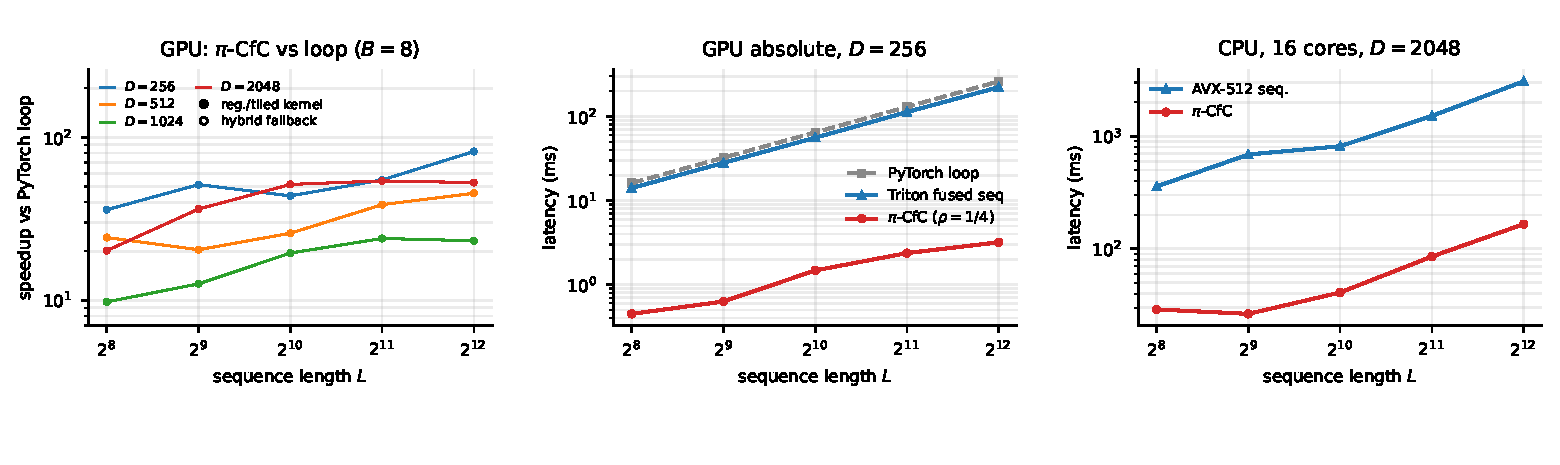
\includegraphics[width=\textwidth]{../figures/fig_hardware_speedup.pdf}
\caption{Left: GPU speedup of $\pi$-CfC over the PyTorch loop versus $L$, one curve per $D$. Middle: absolute
GPU latency at $D=256$ against both sequential baselines. Right: the same comparison on 16 pinned Zen~5 cores,
where our AVX-512 sequential kernel is the baseline to beat.}
\label{fig:hw}
\end{figure}

At $D=256$, $L=1024$, $B=8$ the PyTorch loop takes 64.50~ms, the fused Triton sequential kernel 55.83~ms, and $\pi$-CfC ($\rho=0.0625$) 1.47~ms: 43.7$\times$ and 37.9$\times$.

The largest GPU gain appears at $D=256$, $L=4096$, $B=1$: 109.2$\times$ over the loop and 94.9$\times$ over the fused sequential kernel ($\rho=0.0625$, register-resident kernel).

At $D=512$ the hot set is $d_{\text{hot}}=32$, so the register-resident kernel handles the whole time loop in one launch: 2.53~ms versus 65.38~ms for the loop (25.8$\times$).

At $D=1024$ the hot set is $d_{\text{hot}}=64$, so the register-resident kernel handles the whole time loop in one launch: 3.31~ms versus 64.56~ms for the loop (19.5$\times$).

At a fixed budget of $\rho=1/4$, which is the operating point the accuracy study recommends, the speedup over the loop is uniform across sequence lengths ($D=256$: 21.1--26.9$\times$, $D=512$: 8.5--10.7$\times$, $D=1024$: 2.8--3.5$\times$, $D=2048$: 3.4--3.6$\times$), handled by the L2-fused tiled kernel. Only the $d_{\text{hot}}=512$ rows ($D=1024$, $\rho=1/2$) stay at parity, because a 512-wide register tile doubles the per-step gather work.

At $D=2048$, $L=256$ the best split still gives 20.2$\times$; the $d_{\text{hot}}>512$ rows are the only ones that fall back to the hybrid path, and they are labelled as such in the table.

On the CPU, $\pi$-CfC beats our own AVX-512 sequential kernel in 40 of 60 cells; its best margin is at $D=2048$, $L=4096$, $B=16$ (11.86$\times$: 3183.33~ms versus 268.34~ms), while against the PyTorch loop the best cell reaches 15.4$\times$.

Merging the four CPU stages into one C entry point (\code{picfc\_forward\_fused}) removes the Python/ctypes round trips and wins in 56 of 60 CPU cells; the best is $D=2048$, $L=512$, $B=8$, where it takes 26.44~ms against 687.90~ms for the AVX-512 sequential kernel (26.02$\times$).

The benchmark process itself peaked at \textbf{1609~MB} of \code{RssAnon} over all 60 cells, against a self-imposed 1\,500~MB budget: 34 of the largest cells exceed one micro-batch of the fp32 activation set and were therefore measured one batch row at a time (marked $^{*}$ in the tables), which keeps the CUDA side inside 8~GB but leaves the host holding one $[1,L,D]$ pre-activation triple plus its CPU mirror. That is a real 7\% overshoot on the largest cell, not a rounding artefact, and it is reported rather than hidden: every other stage of the pipeline stayed under 1\,010~MB.


\section{What went wrong first}\label{sec:bugs}

Every number above was re-measured after at least one of the following defects was found; they are listed
because each one changed a published conclusion.

\begin{enumerate}[leftmargin=1.4em]
\item \textbf{Leakage in the ridge study} (metric: parity accuracy $0.848$ for a model that cannot do parity).
      The calibration split was the first half of the \emph{evaluation} batch. With an independently generated
      split, pure-linear scores $0.496$/$0.505$ after ridge, and the shuffled-target control $0.502$.
\item \textbf{Leakage in DAFT} (metric: $+0.62$ $R^2$ on A-oscillator). Fine-tuning used the evaluation batch;
      with fresh sequences the honest gain is $+0.32$.
\item \textbf{One-step lookahead} ($\varepsilon$ growing with $\rho$, $1.88$ relative error at
      $\rho=1$). The cold state fed to the hot gates was $h^{\text{cold}}_t$ instead of $h^{\text{cold}}_{t-1}$.
\item \textbf{Picard double counting} ($\sim10^3\times$ error): the cold refinement added
      $\bar h U^\top$ on top of the exact coupling term.
\item \textbf{Triton precision mismatch}: \code{tl.dot} defaults to tf32, which turned a feedback loop into
      $2.5\times10^{-1}$ relative error; \code{input_precision="ieee"} plus
      \code{allow_tf32=False} on the reference was also needed, since the reference itself deviated by
      $4\times10^{-5}$ under tf32 and masqueraded as kernel error.
\item \textbf{Triton assumes contiguous pointers}: passing \code{gf[:, :, :n\_cold]} views produced silent
      garbage; every kernel argument is now \code{.contiguous()}.
\item \textbf{In-place hot update} in C++: channels updated before their dependents read $h_{t-1}$; fixed by
      computing all three gate vectors into temporaries first ($10$~ms $\to$ $0.6$~ms per call).
\item \textbf{Biased baselines}: a work-inefficient $O(T\log T)$ Hillis--Steele scan as the CPU baseline
      ($169$~ms versus $18$~ms for the work-optimal scan), and a PyTorch GPU loop that recomputed the input
      projection inside the loop.
\end{enumerate}

\section{Discussion}

\paragraph{The honest summary.} The permutation is exact and free; the accuracy it preserves depends on the
task's state complexity and, for stiff systems, on a cheap linear readout recalibration; the speedup depends
on whether the hot weights fit in registers. A deployment recipe follows: use $\rho=1/16\dots1/8$ for
state-tracking tasks, spend 5 epochs of DAFT on the hot block, refit the readout in closed form, and treat
$d_{\text{hot}}>64$ as a different engineering problem (shared memory or a two-level state), not as a tuning
knob. For stiff oscillatory dynamics we recommend \emph{not} decoupling at all until the readout is
recalibrated, and we would not apply the method to a task whose state must survive an arbitrarily long gap
without a write (only the flip-flop class passes that test here).

\paragraph{Threats to validity.} All tasks are synthetic, and $D\le1024$; the CPU comparison is against our own
AVX-512 sequential kernel, which is a strong but not a vendor-optimal baseline; the GPU picture is
register-limited by construction; the three checkpoints are single-seed, so the $\pm$ we report is batch noise,
not training noise.

\section{Reproduction}

\begin{verbatim}
python scripts/phase1_train_and_audit.py          # 3 checkpoints + isomorphism + spectrum
python scripts/phase2_dynamical_equivalence.py    # 6 rules x 8 rho x 3 models + scan gate
python scripts/phase3_expressivity_and_calibration.py amp|ridge|expr|osc
python scripts/phase4_hardware_benchmarks.py full # 60 cells, gated, RSS-probed
python scripts/make_tables.py                     # paper tables from results/*.json
\end{verbatim}

All logs are in \code{results/}; peak \code{RssAnon} stays below 1.0~GB per process once the studies are run
separately, and each kernel is gated against its reference before any timing is recorded.

\end{document}
